% ============================================
\section{Module overview}
% ============================================

\subsection{Module I --- Basic Data}

\begin{frame}[t]{Module I}{Basic Data}
  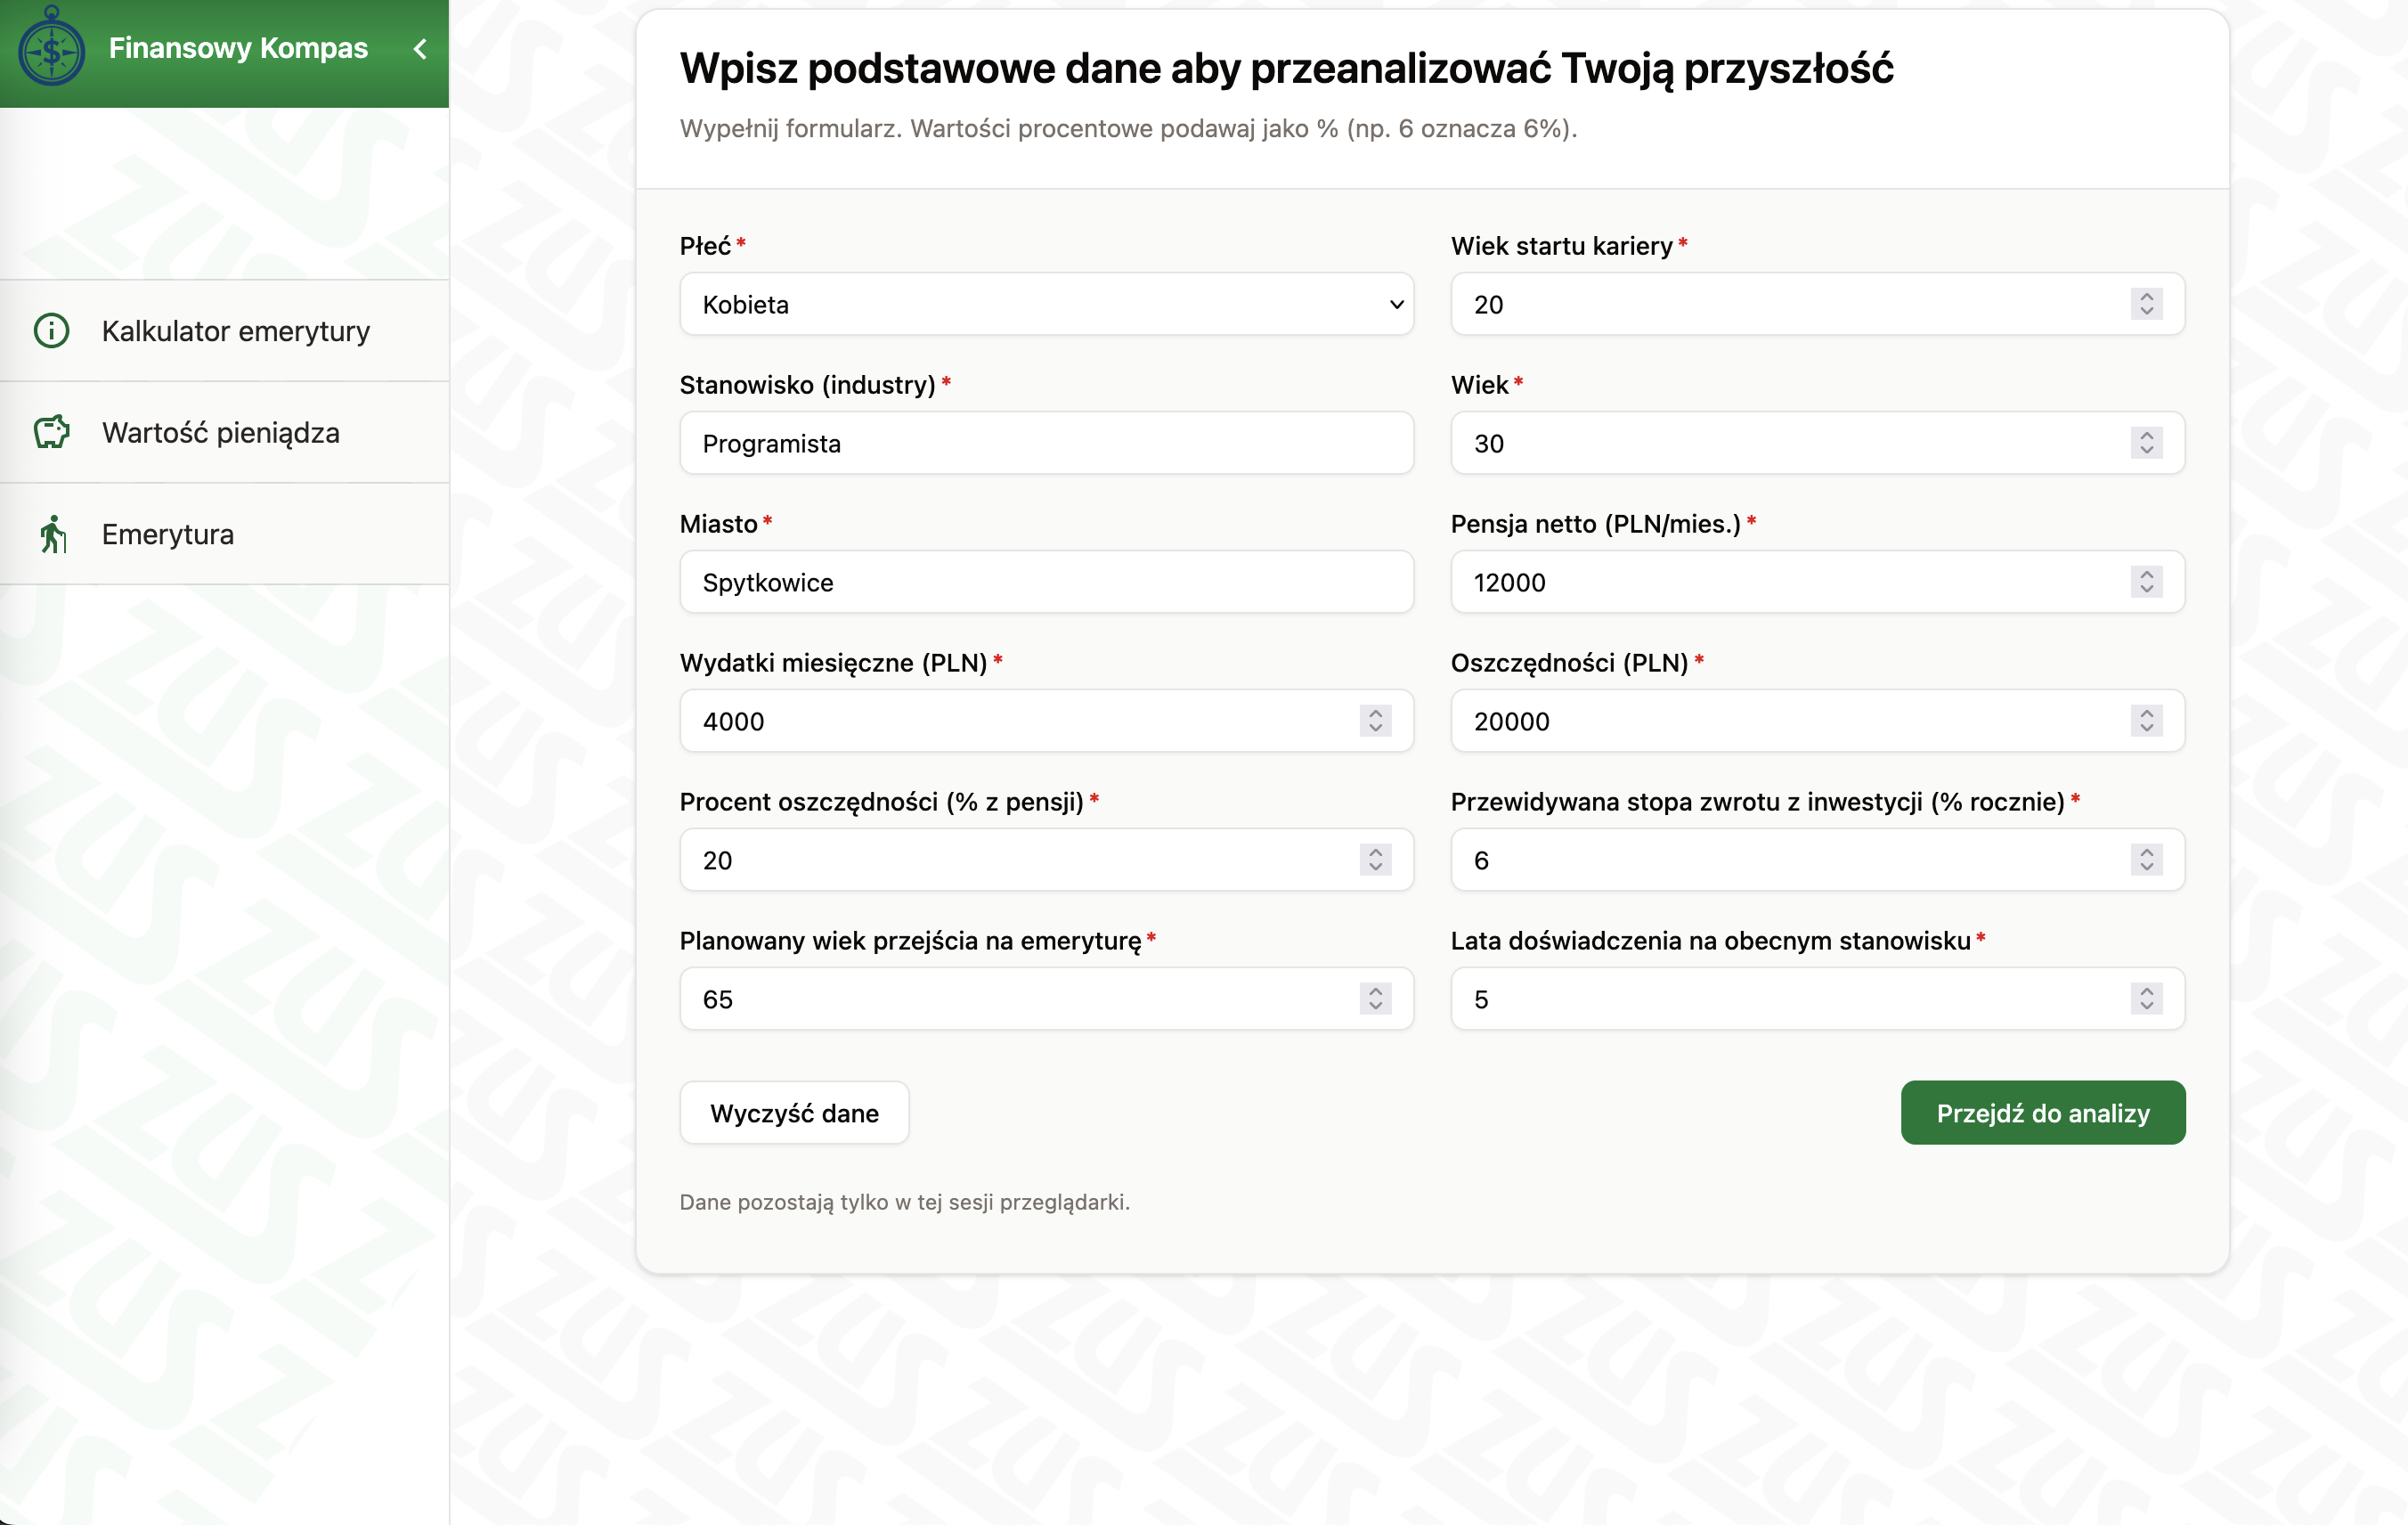
\includegraphics[width=.8\textwidth]{img/module_1_basic_data}
\end{frame}

\begin{frame}[t]{Module I}{Basic Data}
With a minimal set of inputs from the user:
\pause
\begin{itemize}
  \item occupation/industry,
  \pause
  \item place of residence,
  \pause
  \item age,
\end{itemize}
\pause
our system immediately builds a first‑pass financial model:
\begin{itemize}
  \pause
  \item an earnings projection (in nominal and real terms),
  \pause
  \item monthly expenses and savings, years of experience, retirement age —
        all values can be refined manually at any time.
\end{itemize}
\end{frame}

\subsection{Module II --- Simplified Pension Calculator}

\begin{frame}[t]{Module II}{Simplified Pension Calculator}
  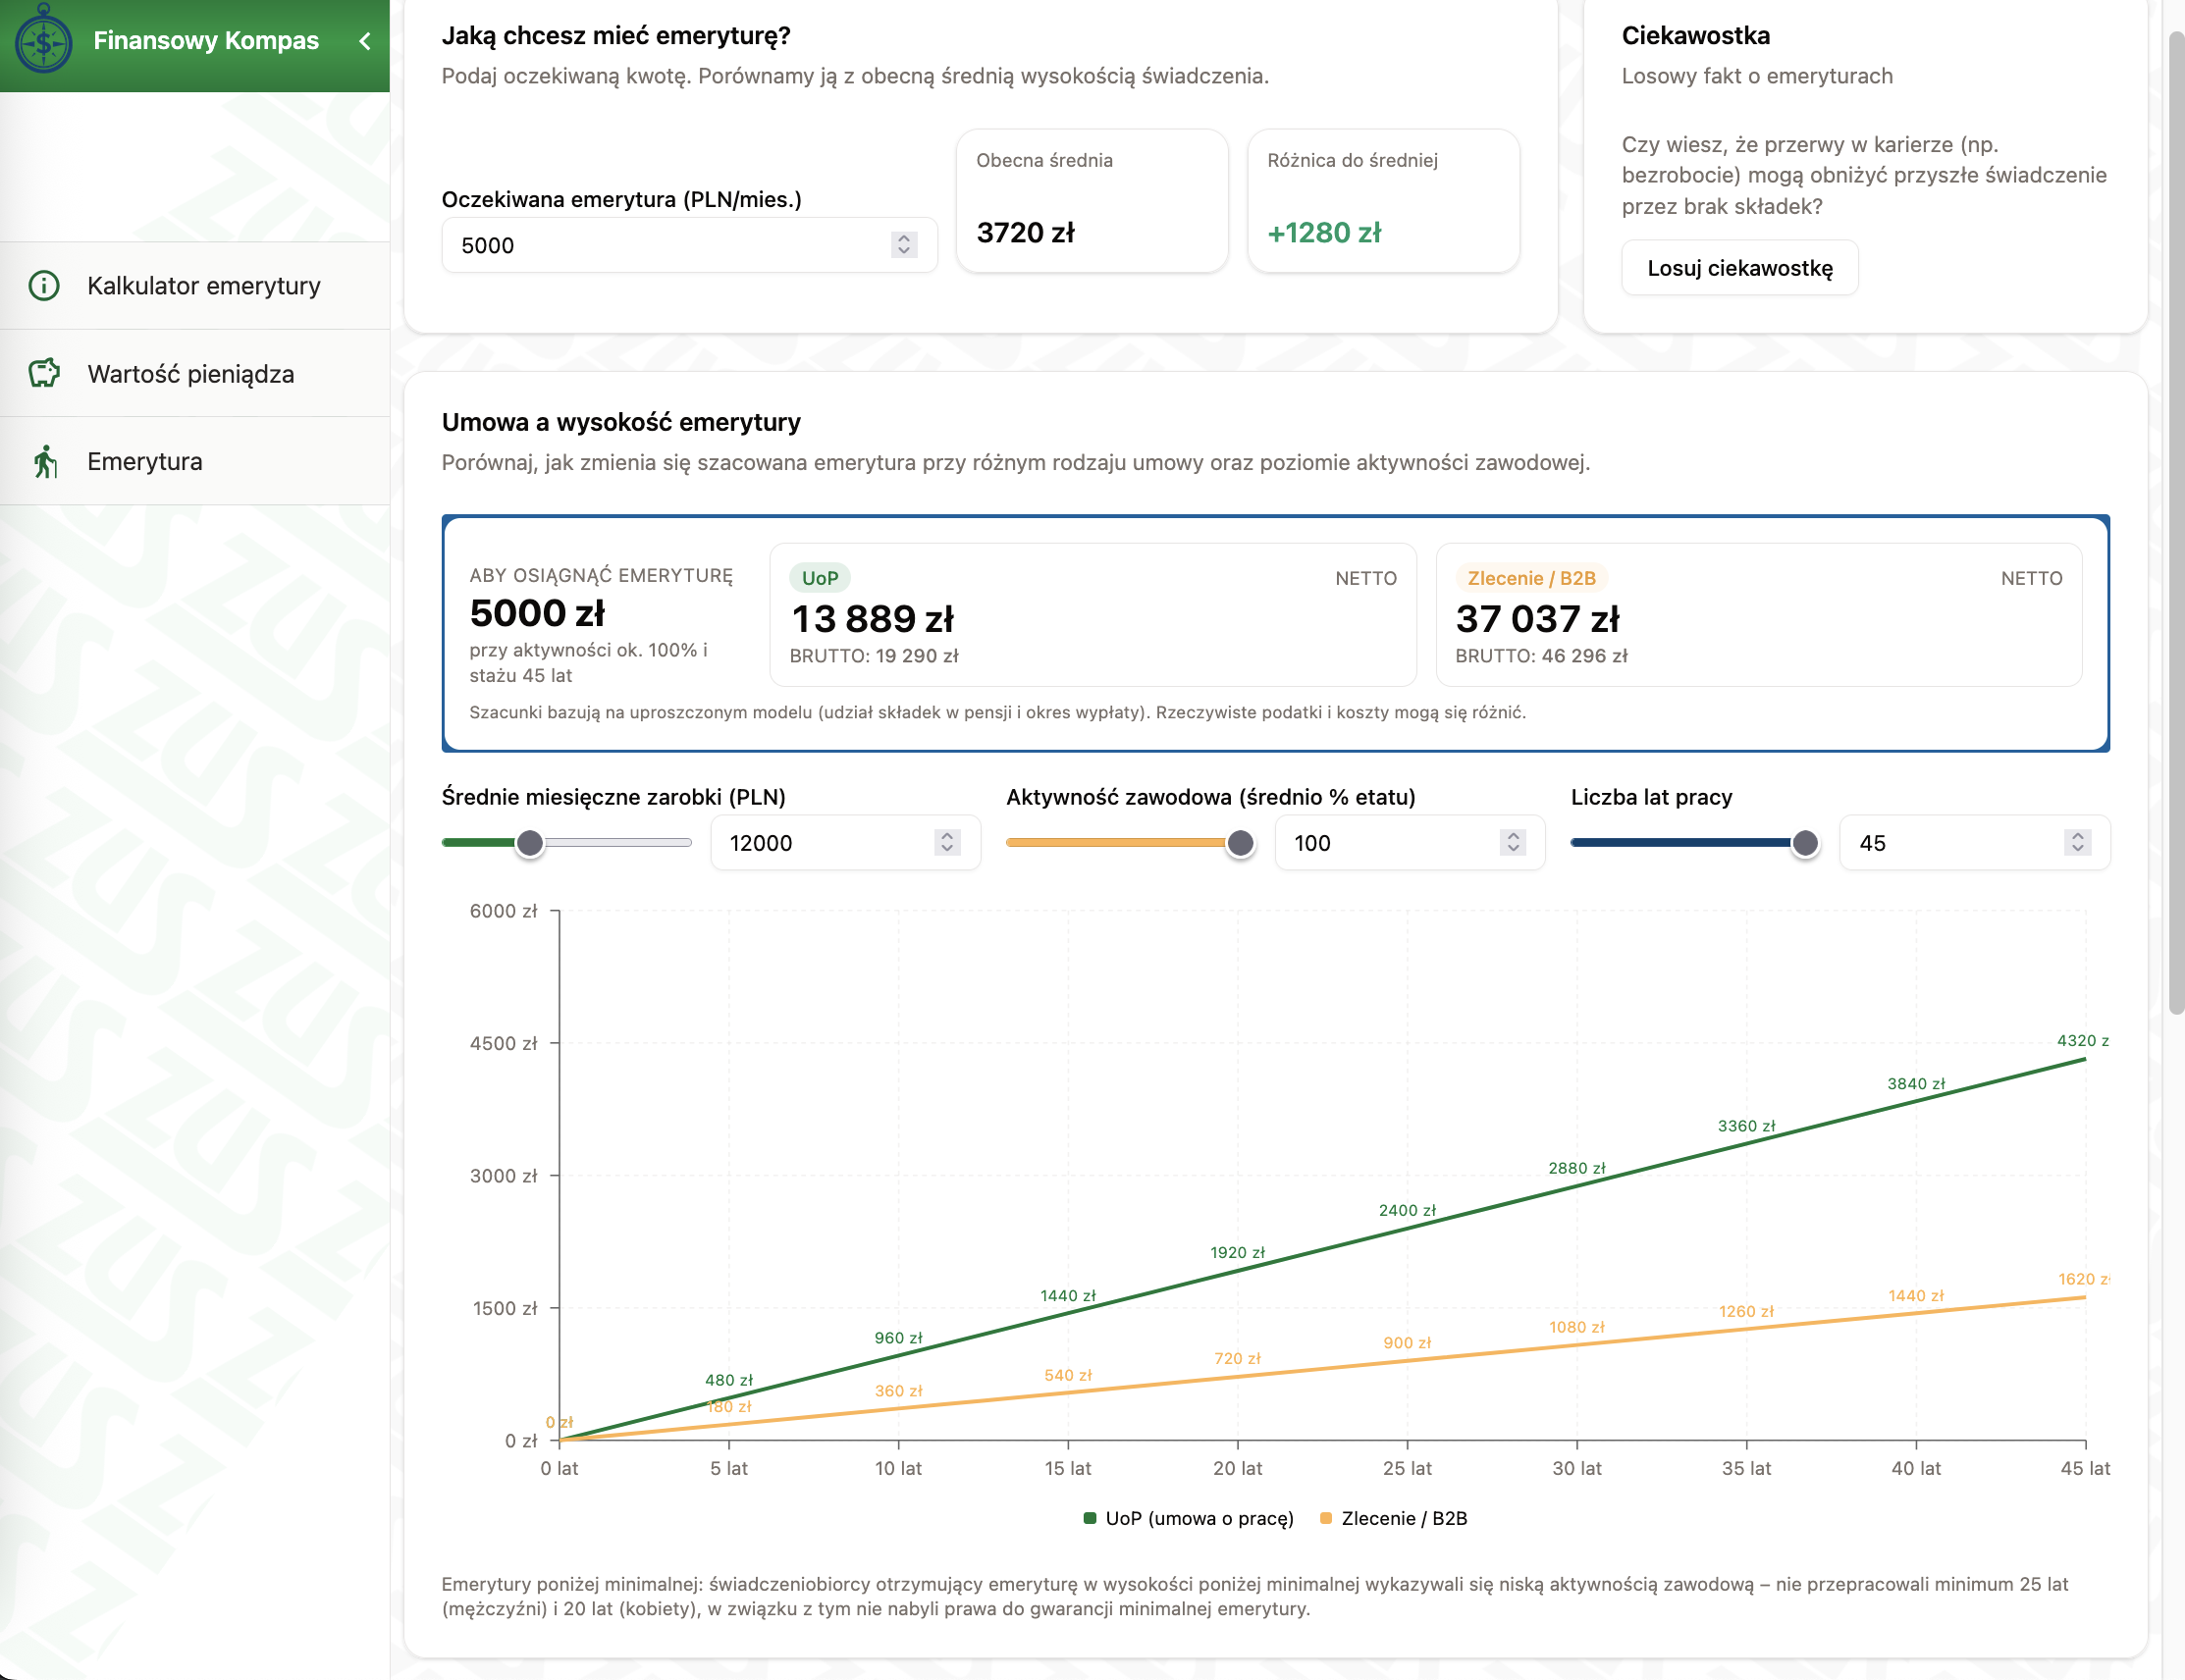
\includegraphics[width=.8\textwidth]{img/module_2_simple_pension_calculator}
\end{frame}

\begin{frame}[t]{Module II}{Simplified Pension Calculator}
A dynamic chart illustrating the relationship between a planned nominal pension and employment history:
\begin{itemize}
  \item average earnings,
  \item length of work experience,
  \item employment fraction (full-time, part-time, etc.)
\end{itemize}
\end{frame}

\begin{frame}[t]{Module II}{Simplified Pension Calculator}
The module also compares the pension of a person employed under an employment contract
with that of a sole proprietor (B2B),
assuming the minimal legally required ZUS contribution.
\end{frame}

\begin{frame}[t]{Module II}{Simplified Pension Calculator}
The module also presents contextual tidbits ---
subtly educating young users about key elements of the pension system.
\end{frame}

\begin{frame}[t]{Module II}{Simplified Pension Calculator}
Additionally: a chart presenting the median pension for ten random occupations.
\\[2em]
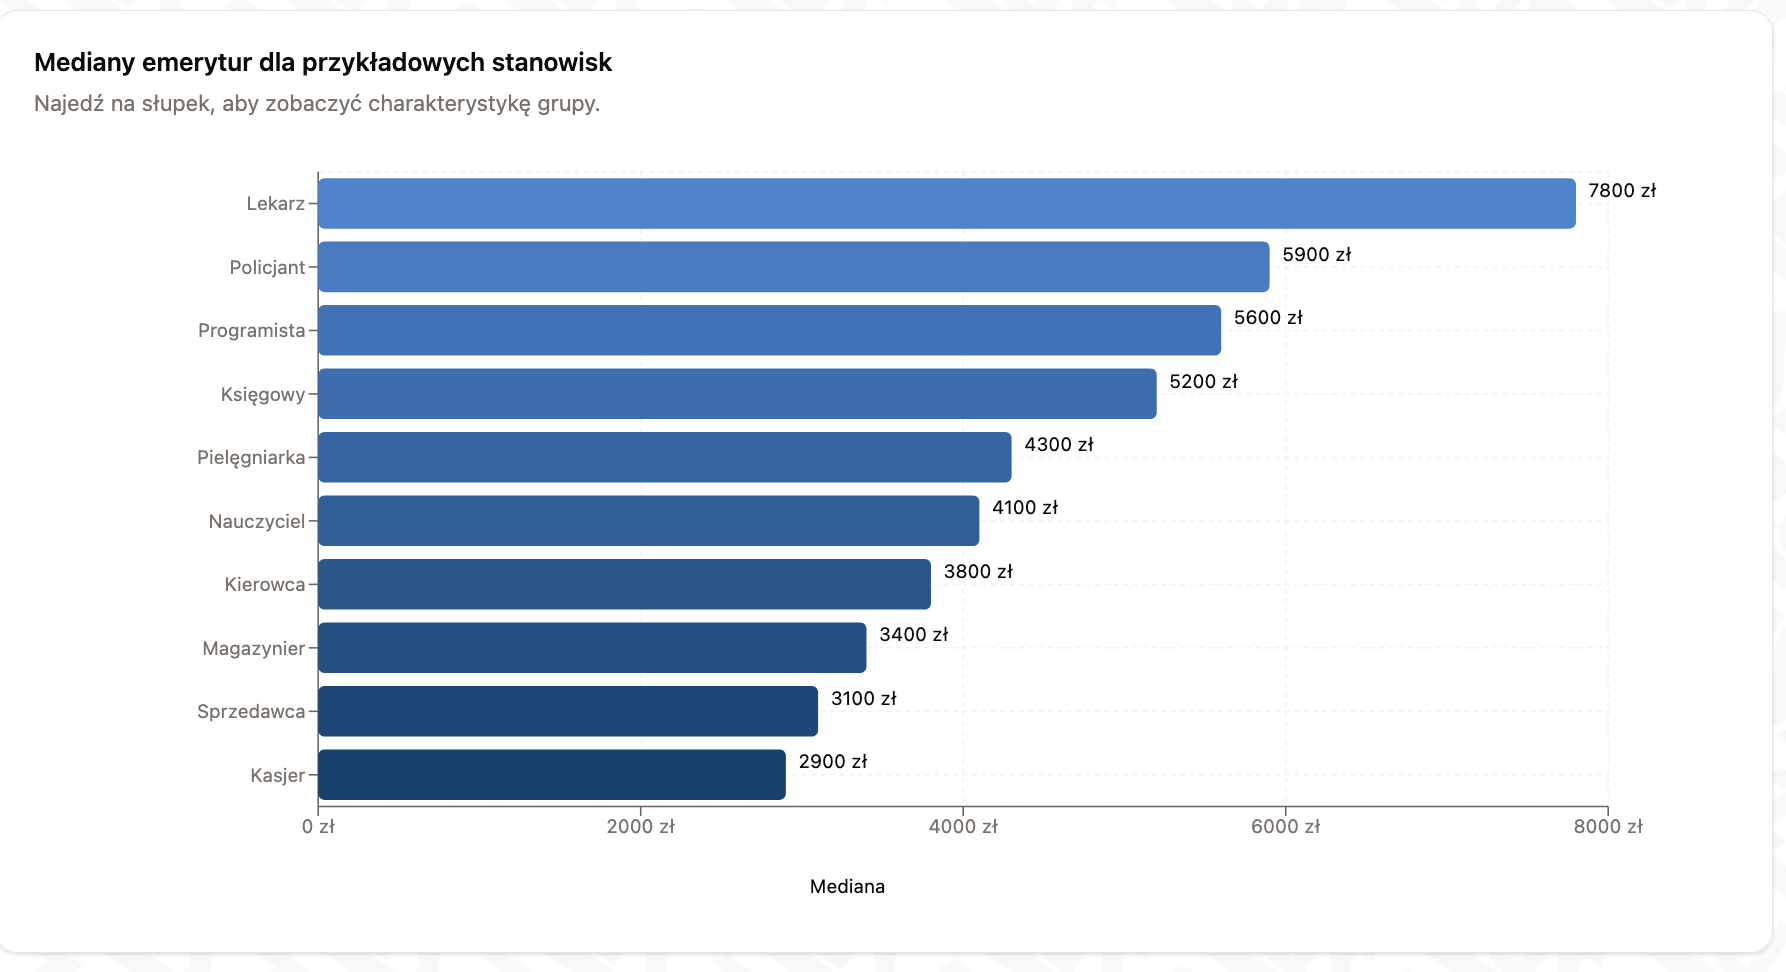
\includegraphics[width=.8\textwidth]{img/module_2b_median_pensions}
\end{frame}

\subsection{Module III --- Value Of Money}

\begin{frame}[t]{Module III}{Value Of Money}
  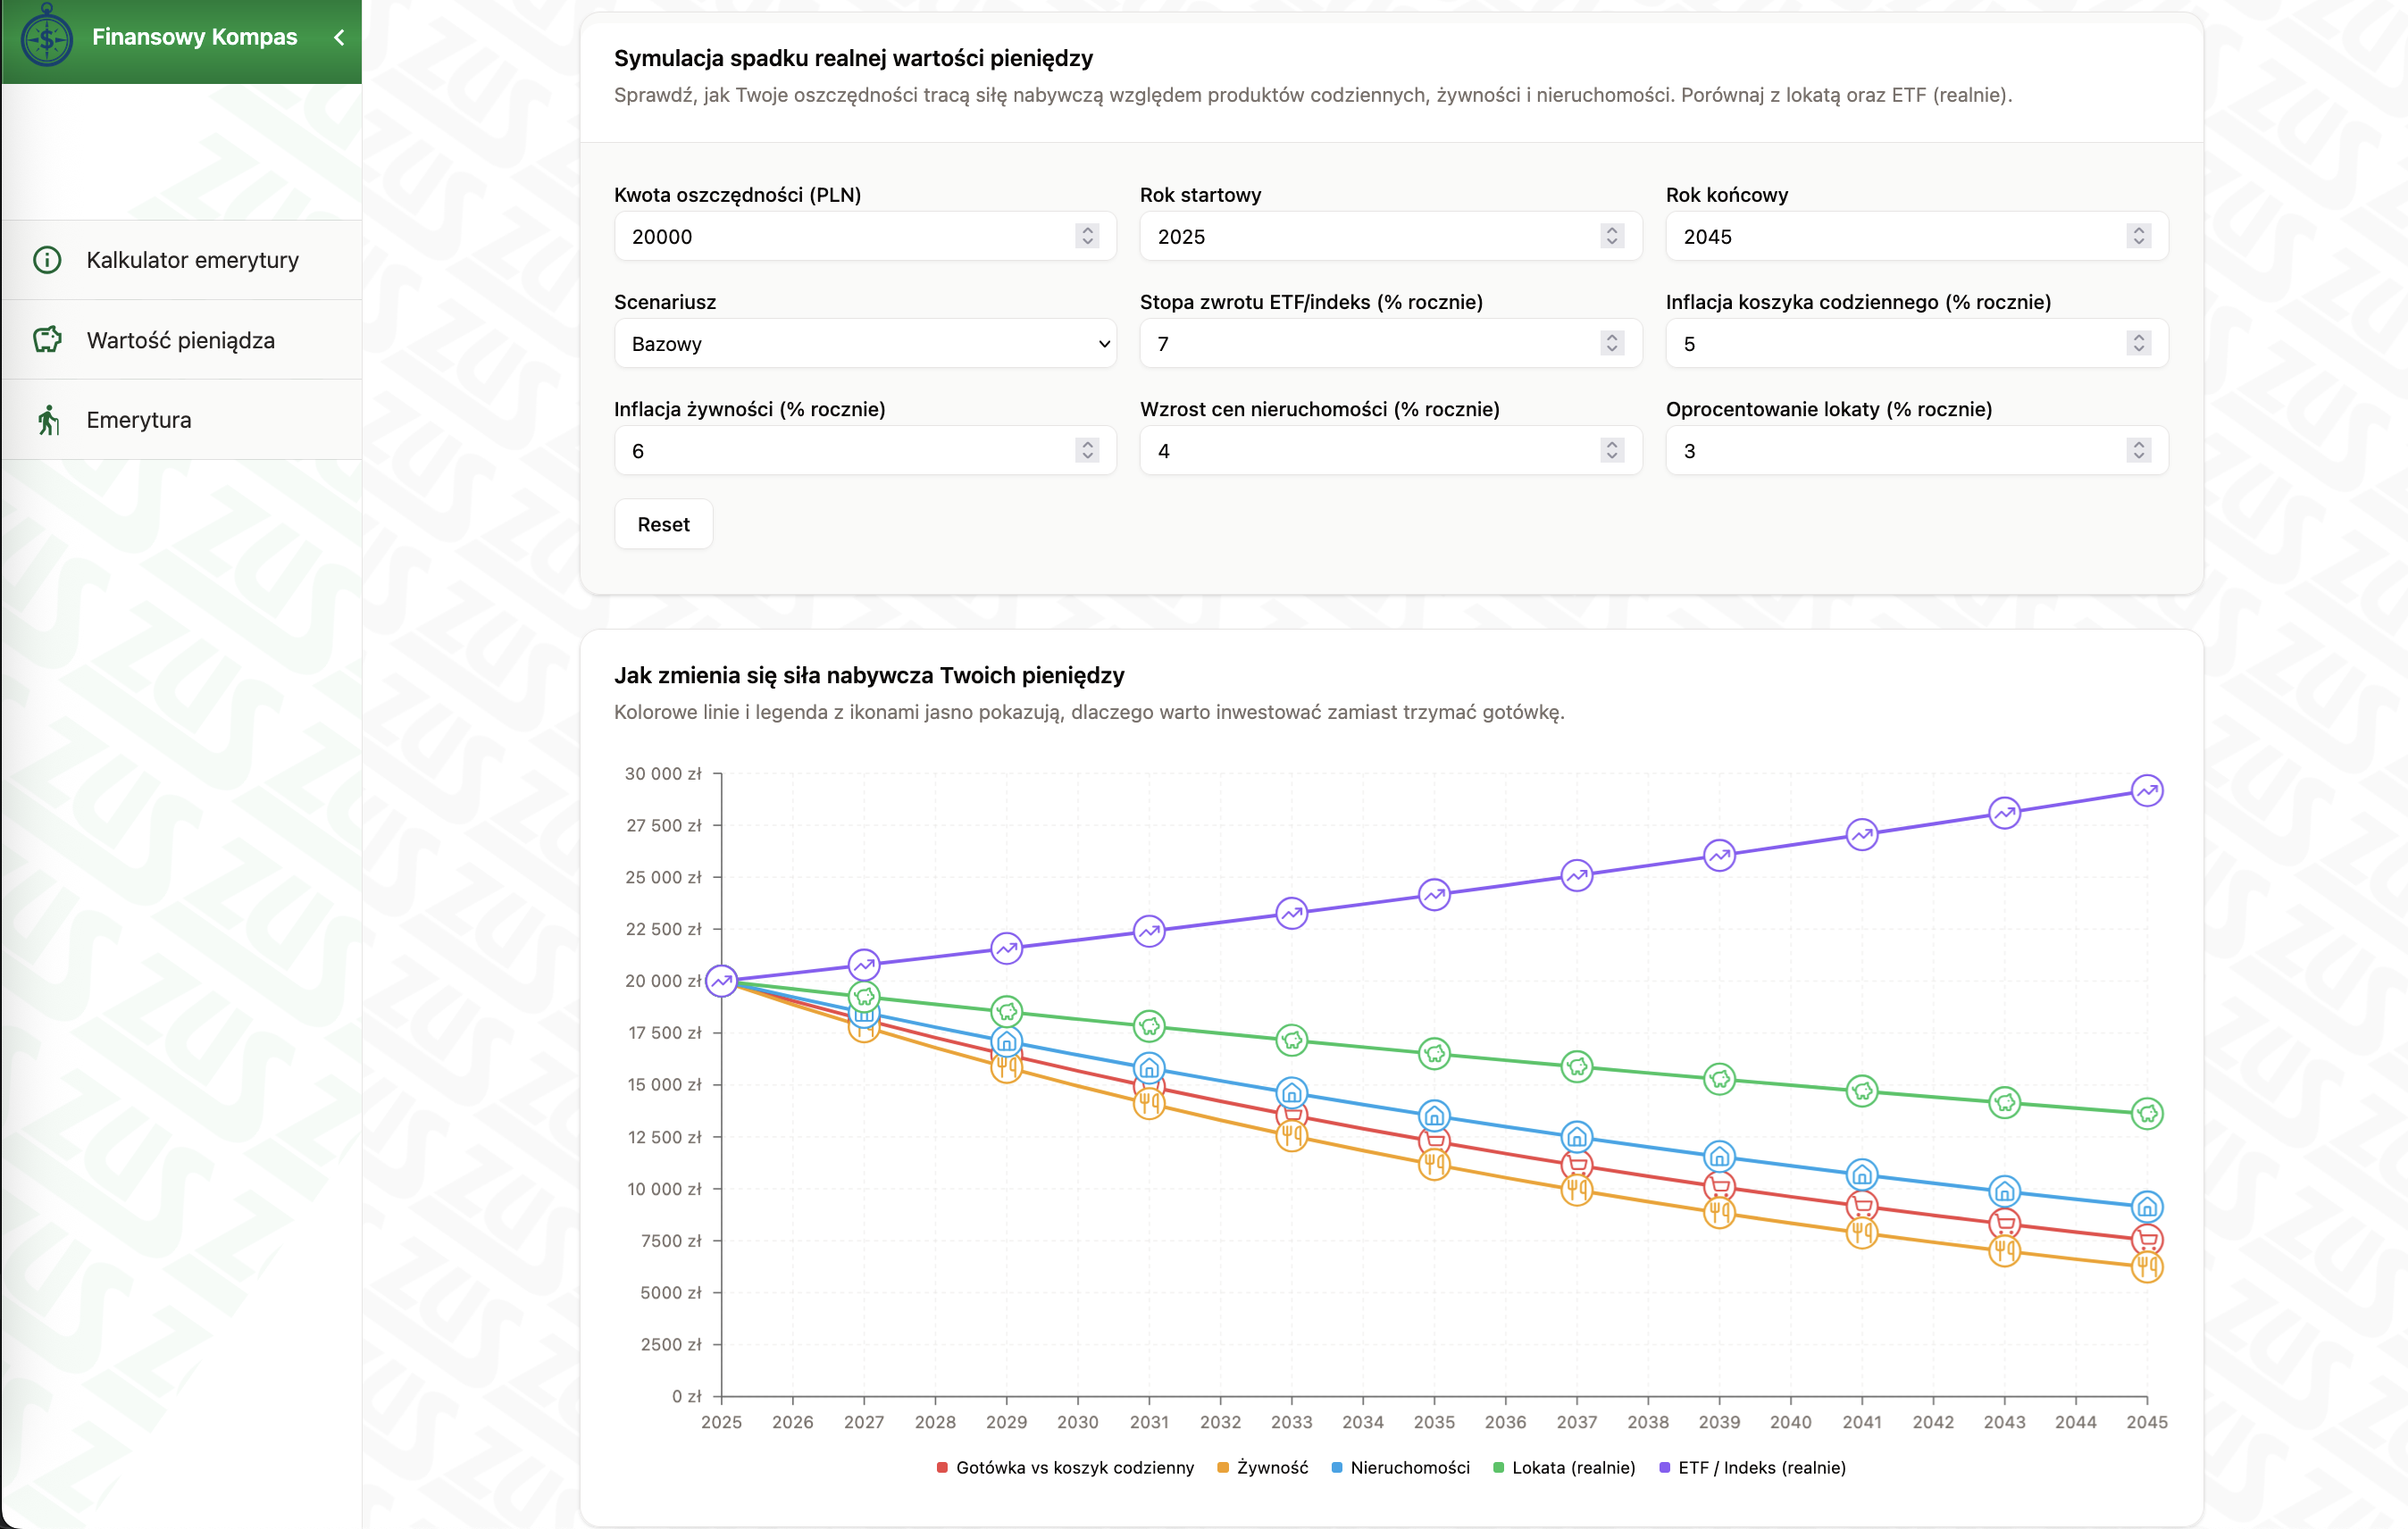
\includegraphics[width=.8\textwidth]{img/module_3_the_value_of_money}
\end{frame}

\begin{frame}[t]{Module III}{Value Of Money}
The goal of the “Value Of Money” module is to make inflation tangible.

\pause
With configurable scenarios the user can observe on a chart
how the value of savings kept in a savings' account or term deposit evolves.
\pause
For comparison, we also include: rising prices of food and real estate,
and data for global equities (a diversified ETF).


\pause For comparison the chart also includes data on
rising prices of essential material goods: food, real estate,
and example data for global equities in the form of a diversified ETF.
\end{frame}

\subsection{Module IV --- Extended Pension Calculator}

\begin{frame}[t]{Module IV}{Extended Pension Calculator}
  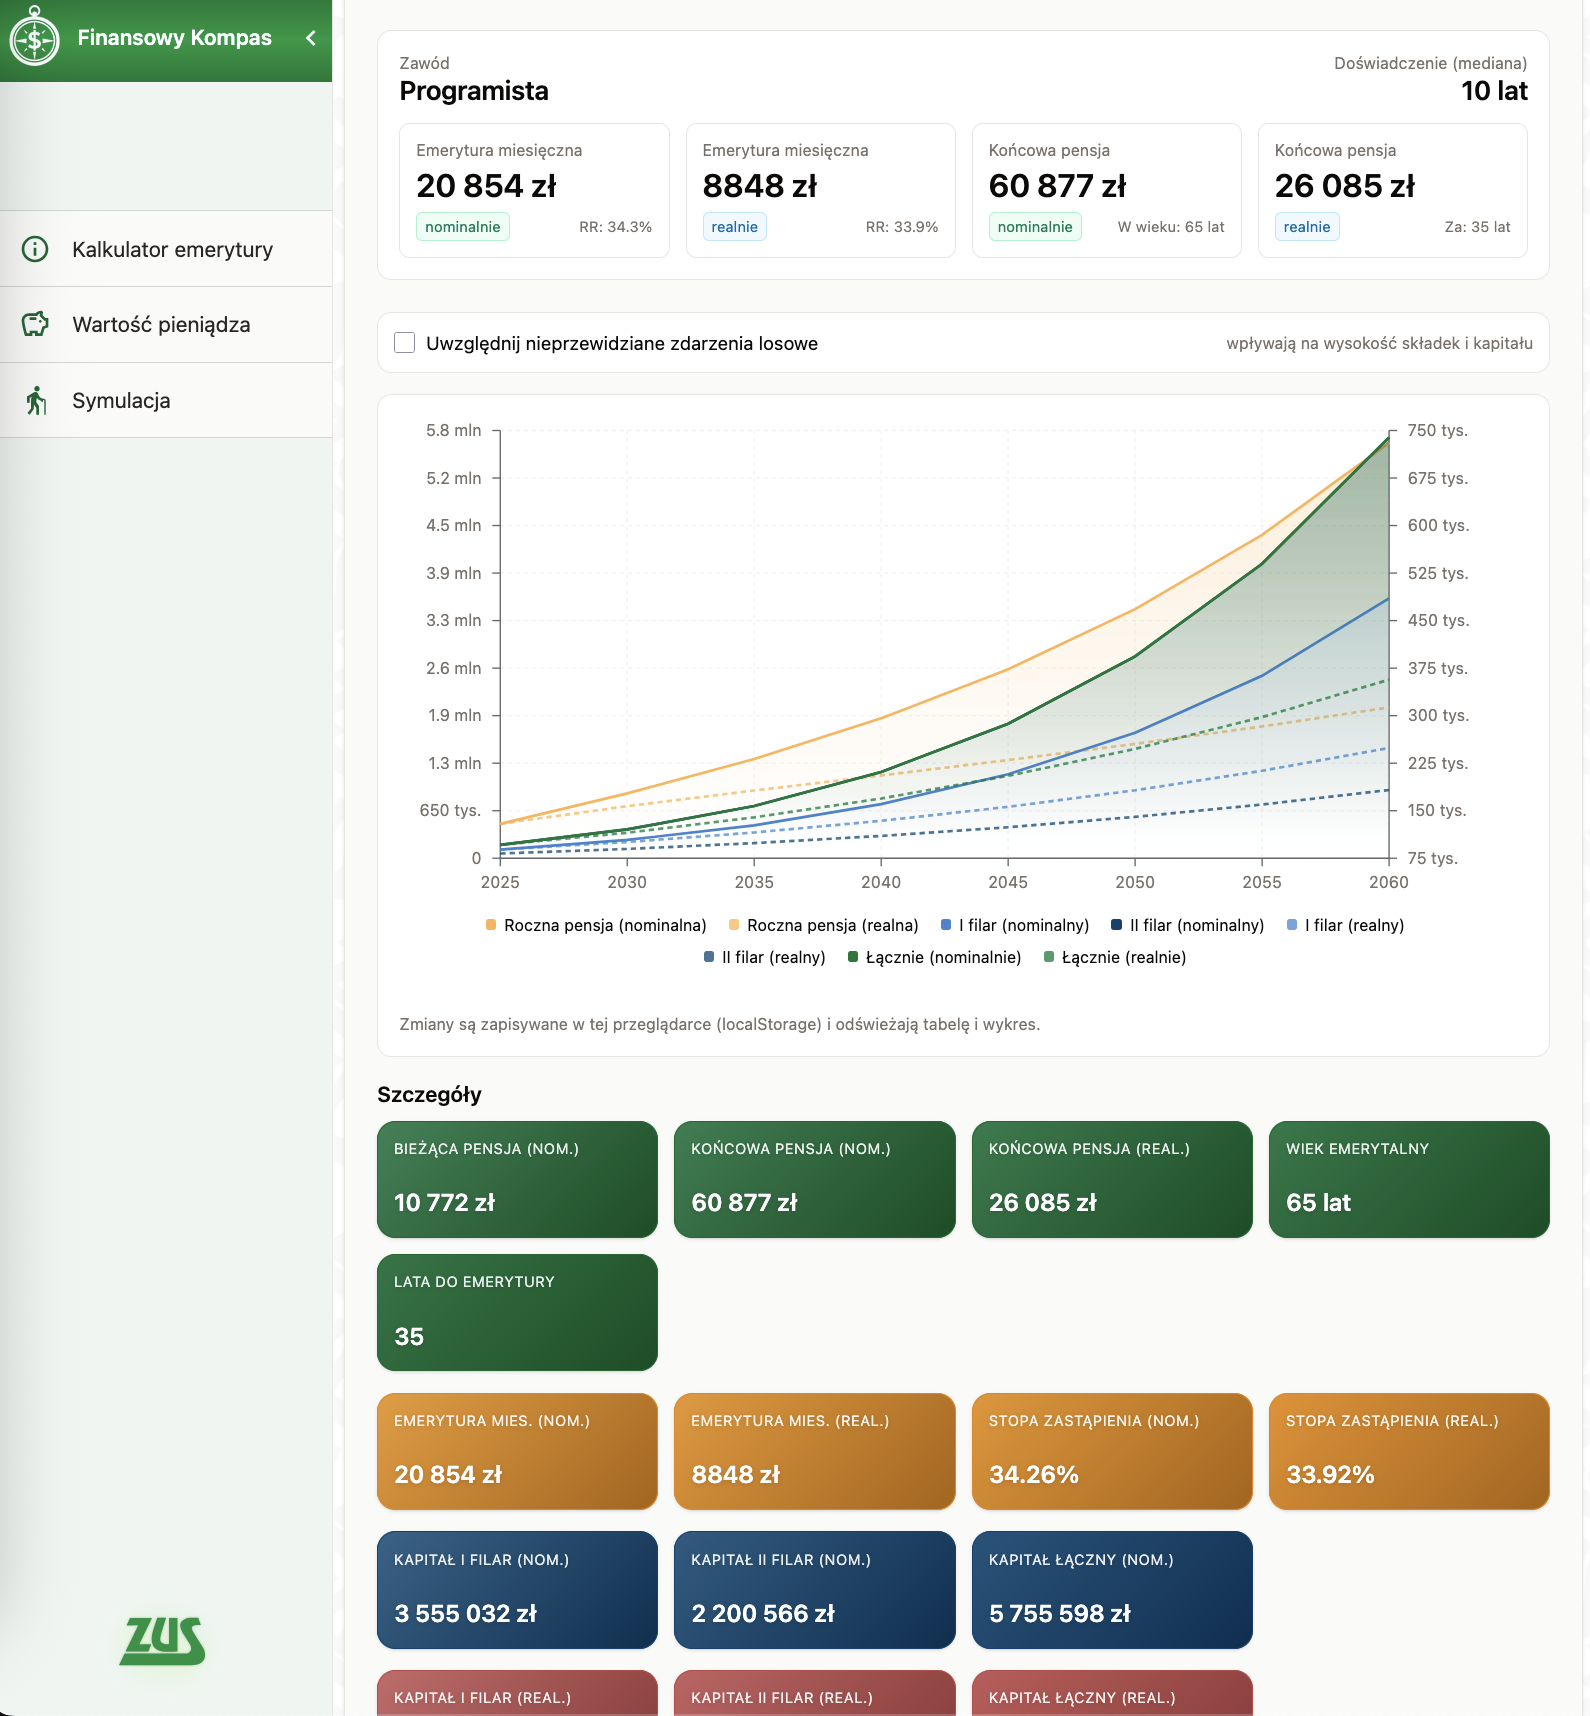
\includegraphics[width=.8\textwidth]{img/module_4_extended_pension_calculator}
\end{frame}

\begin{frame}[t]{Module IV}{Extended Pension Calculator}
We use the full set of user data (entered manually or inferred from models and defaults)
and illustrate the key parameters:
\begin{itemize}
  \pause
  \item funds accumulated in the ZUS account and sub‑account until the end of working life,
  \pause
  \item earnings trajectory, forecast pension value and the replacement rate —
        the real, percentage change in income at the moment of retirement.
\end{itemize}
\end{frame}

\begin{frame}[t]{Module IV}{Extended Pension Calculator}
Unlike Module II, Module IV not only uses the full set of user data
(entered manually or computed from our models and sensible defaults)
but also illustrates all important pension parameters:

\begin{itemize}
    \pause
    \item a chart showing money accumulated in the ZUS account and sub‑account over the remaining working years
    \pause
    \item earnings progression, pension levels and the so‑called replacement rate — the real percentage change
    in income the user will experience at retirement.
\end{itemize}
\end{frame}

\subsection{Module V --- Random Events Simulation}

\begin{frame}[t]{Module V}{Random Events Simulation}
  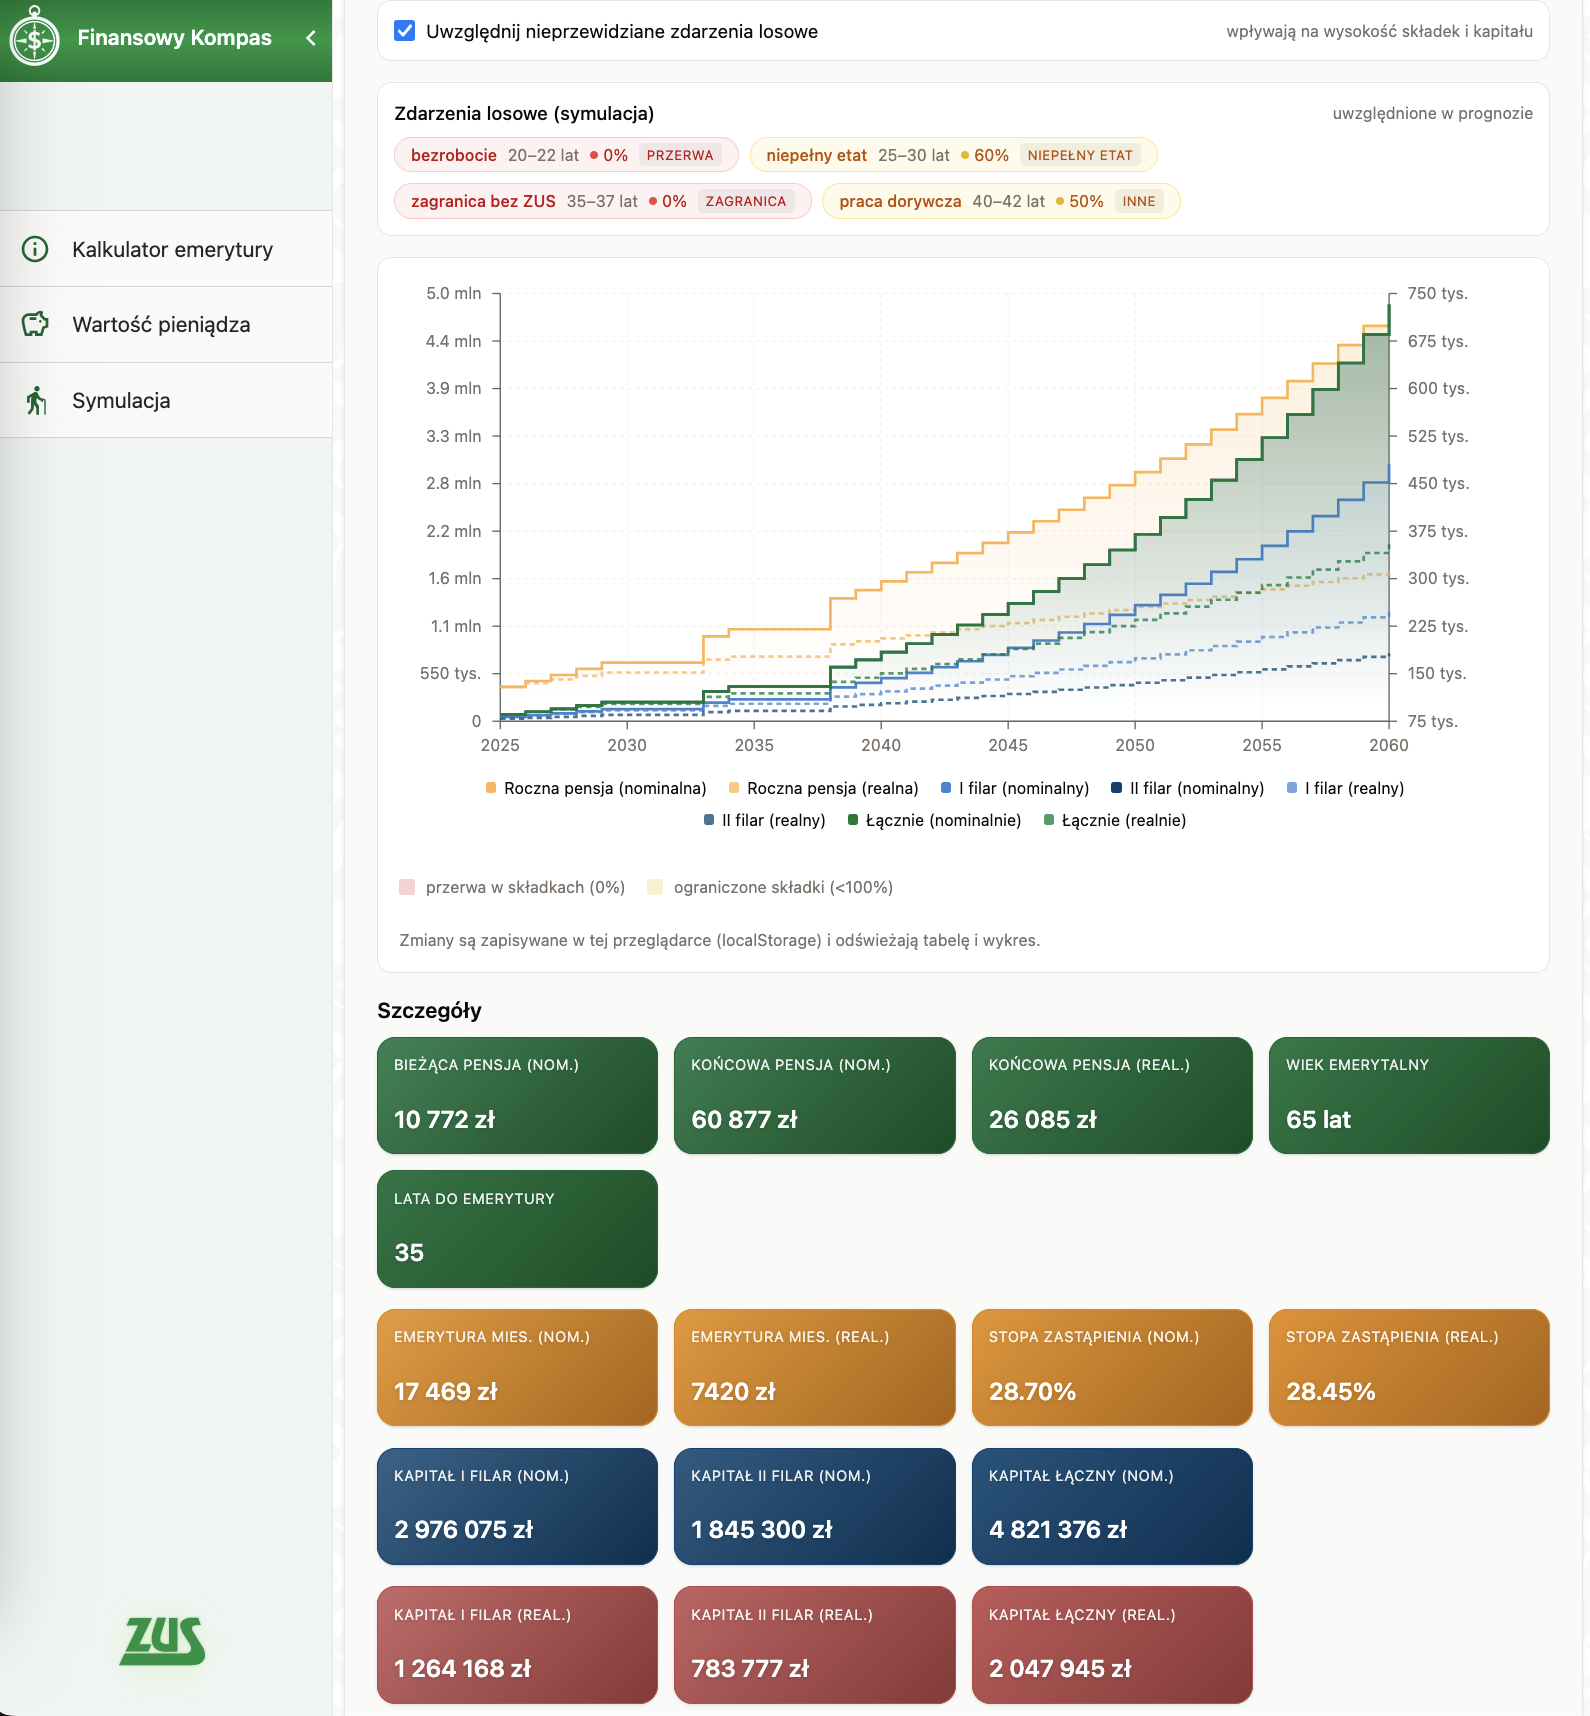
\includegraphics[width=.8\textwidth]{img/module_5_random_events}
\end{frame}

\begin{frame}[t]{Module V}{Random Events Simulation}
An optional module that factors random events (job loss, illness, parental leave, etc.)
into the calculations of Module IV.
\pause
It helps users understand how strongly early breaks in employment and contributions
can affect the final pension amount.
\end{frame}

\subsection{Module VI --- Collecting Statistics And Generating An .xlsx Report}

\begin{frame}[t]{Module VI}{Collecting statistics and generating a report}
At the hackathon stage we did not introduce authentication or a database,
but we implemented a module for collecting anonymous statistics,
available as an Excel (.xlsx) report to the site administrator,
in line with the task requirements.
\end{frame}
